\section{Reducción de Datos}


\begin{definición}[Estadístico suficiente]
	Sea $(\Omega, \mathcal{A}, \mathcal{P})$ el espacio probabilístico asociado a un experimento aleatorio $\mathcal{E}$, una variable aleatoria observable $X: \Omega \longrightarrow \mathbb{R}$ y su modelo estadístico asociado ( $\left.\chi, \mathcal{B}, F_{\theta}\right)_{\theta \in \Theta \subset \mathbb{R}^{\ell}}, \mathcal{B}=\mathcal{B}(\mathbb{R})$, y $\left(X_{1}, \cdots X_{n}\right)$ m.a.s. $(n) \sim X$\\
	$T: \mathbb{R}^n \to \mathbb{R}^m$ es un estadístico suficiente para $\theta$ cuando $\forall (x_1, \ldots, x_n) \in \Omega$ se cumple que: 
	$$P(X_1 = x_1, \ldots, X_n = x_n | T = t) \text{	 no depende de } \theta \quad \forall t \in \mathbb{R}^m$$
\end{definición}


\ejemplo{
	Sabiendo que $X \sim Bin(1, \theta)$, veamos si se cumple que el estadístico $T = \sum_{i = 1}^{n} X_i$ es suficiente para $\theta$\\
	Tenemos que:
	$$X_i \sim Bin(1, \theta) \implies T = \sum_{i = 1}^n X_i \sim Bin(n, \theta)$$
	Para saber si un estadístico es suficiente necesitamos además la funcion de distribucion de la muestra, que en este caso: 
	$$X_i \sim Bin(1, \theta) \equiv Bernoulli(\theta)$$ $$\implies P(X_1 = x_1, \ldots, X_n = x_n) = \prod_{i = 1}^{n} \theta^{x_i} (1 - \theta)^{1 - x_i} = \theta^{\sum_{i = 1}^{n} x_i} (1 - \theta)^{n - \sum_{i = 1}^{n} x_i} \prod_{i = 1}^{n}$$
	Para ver si es suficiente, necesitamos calcular la probabilidad condicionada de la muestra dado el estadístico, que en este caso es:
	$$P(X_1 = x_1, \ldots, X_n = x_n | \sum_{i = 1}^{n} X_i = t) = \frac{P(X_1 = x_1, \ldots, X_n = x_n)}{P(\sum_{i = 1}^{n} X_i = t)} = \frac{\theta^{\sum_{i = 1}^{n} x_i} (1 - \theta)^{n - \sum_{i = 1}^{n} x_i}}{\binom{n}{t} \theta^t (1 - \theta)^{n - t}} = \frac{1}{\binom{n}{t}}$$
}
  
\subsection{Teorema de Factorización de Fisher}
  
\begin{teorema}[de Factorización de Fisher (Caracterización de estadísticos suficientes)]
	$T=T\left(X_{1}, \cdots X_{n}\right): \mathbb{R}^{n} \longrightarrow \mathbb{R}^{m}$ es un estadístico suficiente para $\theta$ sí y sólo sí existen funciones reales positivas $h: \mathbb{R}^{n} \longrightarrow \mathbb{R}$ y $g_{\theta}: \mathbb{R}^{m} \longrightarrow \mathbb{R}$ tales que $f_{\theta}\left(x_{1}, \ldots, x_{n}\right)=h\left(x_{1}, \ldots, x_{n}\right) g_{\theta}\left(T\left(x_{1}, \ldots, x_{n}\right)\right)$, donde $f_{\theta}\left(x_{1}, \ldots, x_{n}\right)$ es la función de densidad o de masa de la muestra
\end{teorema}
  
  
\begin{proof}
	Esta demostración se desarrolla tomando el caso en el que $X$ sea una v.a. discreta. 
	\begin{itemize}
		\item $(\Rightarrow):$ Supongamos que $T$ es suficiente, entonces como la distribución de la muestra condicionada al estadístico no depende de $\theta$, podemos escribir:
		      $$ f_{\theta}(x_1, \ldots, x_n | t) = \frac{f_{\theta}(x_1, \ldots, x_n)}{f_{\theta}(t)} \text{es independiente de } \theta$$
		      $$\implies f_{\theta}(x_1, \ldots, x_n) = f_{\theta}(t) \cdot f_{\theta}(x_1, \ldots, x_n | t) \implies$$
		      Simplemente tomamos $h(x_1, \ldots, x_n) = f_{\theta}(t)$ y $g_{\theta}(t) = f_{\theta}(x_1, \ldots, x_n | t)$
		\item $(\Leftarrow)$: Supongamos que $f_{\theta}(x_1, \ldots, x_n) = h(x_1, \ldots, x_n) \cdot g_{\theta}(T(x_1, \ldots, x_n))$, entonces:\\
		      $$ f_{\theta}(x, \ldots, x_n | t = T(x_1, \ldots, x_n)) = \frac{f_{\theta}(x_1, \ldots, x_n)}{f_{\theta}(t)} = \frac{f_{\theta}(x_1, \ldots, x_n)}{\sum_{(y_1, \ldots, y_m) : T(y_1, \ldots, y_n) = t} f_{\theta}(y_1, \ldots, y_n)} = $$ $$ = \frac{h(x_1, \ldots, x_n) \cdot g_{\theta}(t)}{\sum_{(y_1, \ldots, y_m) : T(y_1, \ldots, y_n) = t} h(y_1, \ldots, y_n) \cdot g_{\theta}(t)} = \frac{h(x_1, \ldots, x_n)}{\sum_{(y_1, \ldots, y_m) : T(y_1, \ldots, y_n) = t} h(y_1, \ldots, y_n)}$$ La cual es una expresión no dependiente de $\theta$, por lo que $T$ es suficiente.
	\end{itemize}
\end{proof}

\begin{proposición}
	Si $T$ es suficiente para $\theta$ y $S$ es una biyección, entonces $S(T)$ es suficiente para $\theta$
\end{proposición}

\begin{proposición}
	Si $T$ es suficiente para $\theta$ y $S$ es una función medible (en estadística-integrable), entonces $S(T)$ es suficiente para $\theta$
\end{proposición}

\begin{proposición}
	Ssea $X$ variable aleatoria, con $\sigma$ y $\delta$ parámetros, entonces si $T_1$ es suficiente para $\sigma$ y $T_2$ es suficiente para $\delta$ $\iff$ $T = (T_1, T_2)$ es suficiente para $(\sigma, \delta)$
\end{proposición}

\subsection{Ejemplos de Factorización de Fisher}

\ejemplo{
	Veamos si $\theta$ es un parámetro suficiente para el ejemplo anterior, utilizando la Factorización de Fisher.\\
	Como $X \sim \text{Bin}(1, \theta) \equiv \text{Bernoulli}(\theta)$, tenemos que la función de verosimilitud es:
	\[
		f_{\theta}(x_1, \ldots, x_n) = \prod_{i=1}^{n} \theta^{x_i} (1 - \theta)^{1 - x_i} \cdot I_{\{0,1\}}(x_i),
	\]
	donde $I_{\{0,1\}}(x_i)$ es la función indicadora que asegura que $x_i \in \{0, 1\}$. Esto se puede escribir como:
	\[
		f_{\theta}(x_1, \ldots, x_n) = \theta^{\sum_{i=1}^{n} x_i} (1 - \theta)^{n - \sum_{i=1}^{n} x_i} \prod_{i=1}^{n} I_{\{0,1\}}(x_i).
	\]
	Por lo que tomando $h(x_1, \ldots, x_n) = \prod_{i = 1}^{n} I_{\{0,1\}}(x_i)$ y $g_{\theta}(T(x_1, \ldots, x_n)) = \theta^t (1 - \theta)^{n - t}$, tenemos que $T = \sum_{i=1}^{n} X_i$ es un estadístico suficiente para $\theta$.
}

\ejemplo{
	Sea $X \sim Poisson(\theta)$ veamos si el estadístico $T = \sum_{i = 1}^{n} X_i$ es suficiente para $\theta$\\
	Calculemos primero la función de densidad asociada a la muestra: 
	$$X_i \sim Poisson(\theta) \implies f_{x_i}(x_i) = \frac{e^{-\theta} \theta^{x_i}}{x_i!} \implies f_{\theta}(x_1, \ldots, x_n) = \prod_{i = 1}^{n} \frac{e^{-\theta} \theta^{x_i}}{x_i!} = e^{-n\theta} \theta^{\sum_{i = 1}^{n} x_i} \prod_{i = 1}^{n} \frac{1}{x_i!}$$
	Por lo que tomando $h(x_1, \ldots, x_n) = \prod_{i = 1}^{n} \frac{1}{x_i!}$ y $g_{\theta}(T(x_1, \ldots, x_n)) = e^{-n\theta} \theta^t$ demostramos que $T(x_1, \ldots, x_n) = \sum_{i = 1}^{n}$ es un estadístico suficiente para $\theta$
}

\ejemplo{
	Supongamos que tenemos un estadístico $T$ suficiente para el parámetro $\theta$ y una biyección $S$, demostremos que $S(T)$ también es suficiente para $\theta$\\
	Por el Teorema de Caracterización de Fisher tenemos que: 
	$$f_{\theta}(x_1, \ldots, x_n) = h(x_1, \ldots, x_n) \cdot g_{\theta}(T(x_1, \ldots, x_n))$$ para alguna función $h$ y $g_{\theta}$\\ 
	$$\iff f_{\theta}(x_1, \ldots, x_n) = h(x_1, \ldots, x_n) \cdot g_{\theta}(S^{-1}(S(T(x_1, \ldots, x_n))))$$ $$ \iff f_{\theta}(x_1, \ldots, x_n) = h(x_1, \ldots, x_n) \cdot g'_{\theta}(S(T(x_1, \ldots, x_n))) \implies$$
	Entones por el Teorema de Caracterización de Fisher, $S(T)$ es suficiente para $\theta$
}

\ejemplo{
	Veamos si $T = \bar{X} = \sum_{i = 1}^{n}X_i$ es suficiente para $\mu$ si $X \sim N(\mu, \sigma_0)$ con $\sigma_0$ conocida:\\
	$$X_i \sim N(\mu, \sigma_0) \implies f_{\mu}(x) = \frac{1}{\sigma_0 \sqrt{2\pi}} e^{-\frac{1}{2\sigma_0^2}(x - \mu)^2}$$
	$$\implies T = \bar{X} \implies f_{\mu}(x_1, \ldots, x_n) = \prod_{i = 1}^{n} \frac{1}{\sigma_0 \sqrt{2\pi}} e^{-\frac{1}{2\sigma_0^2}(x_i - \mu)^2} = \left(\frac{1}{\sigma_0 \sqrt{2\pi}}\right)^n e^{-\frac{1}{2\sigma_0^2}\sum_{i = 1}^{n}(x_i - \mu)^2}$$
	$\implies$ Tomando $h(x_1, \ldots, x_n) = \left(\frac{1}{\sigma_0 \sqrt{2\pi}}\right)^n$ y $g_{\mu}(T(x_1, \ldots, x_n)) = e^{-\frac{1}{2\sigma_0^2}\sum_{i = 1}^{n}(x_i - \mu)^2}$, tenemos que $T = \bar{X} = \sum_{i = 1}^{n}X_i$ es suficiente para $\mu$
}

\ejemplo{
	Sea el estadístico $T = \left(\sum_{i = 1}^{n}X_i, \sum_{i = 1}^{n} X_i^2 \right)$ suficiente para $\theta = (\mu, \sigma)$ si $X \sim N(\mu, \sigma)$ con $\mu$ y $\sigma$ desconocidas. Veamos si $\left(\bar{X}, S_n^2\right)$ también es suficiente para $\theta$: \\
	$$\bar{X} = \frac{1}{n} \sum_{i = 1}^{n} X_i \quad S_n^2 = \frac{1}{n - 1} \left(\sum_{i = 1}^{n} X_i^2 - n\bar{X}^2\right) \implies$$
	
	$$\text{Sea la biyección } S: \mathbb{R}^2 \to \mathbb{R}^2 \text{ dada por } S(x,y) = \left(\frac{1}{n}x, \frac{1}{n-1}\left(y - \frac{1}{n}x^2\right)\right) \implies$$ 
	
	
	$$ S(T = \left(\sum_{i = 1}^{n}X_i, \sum_{i = 1}^{n} X_i^2 \right)) = \left(\frac{1}{n}\sum_{i = 1}^{n}X_i, \frac{1}{n-1}\sum_{i = 1}^{n}X_i^2 - \bar{X}^2\right) = \left(\bar{X}, S_n^2 \right)$$
	Entonces por el Teorema de Caracterización de Fisher, $\left(\bar{X}, S_n^2\right)$ es suficiente para $\theta$
}

\ejemplo{
	Si $X \sim U(0, \theta)$, veamos si el estadístico $T = (X_{(1)}, X_{(n)})$ es suficiente para $\theta$:\\
	$$ X \sim U(0, \theta) \implies f_{\theta}(x) = \frac{1}{\theta} \cdot I_{(0, \theta)}(x) \implies f_{\theta}(x_1, \ldots, x_n) = \prod_{i = 1}^{n} \frac{1}{\theta} \cdot I_{(0, \theta)}(x_i) = \frac{1}{\theta^n} \cdot I_{(0, \theta)}(X_{(1)}) \cdot I_{(0, \theta)}(X_{(n)})$$
	$$\implies \text{Tomando } h(x_1, \ldots, x_n) = 1  \text{ y } g_{\theta}(T(x_1, \ldots, X_n)) = \frac{1}{\theta^n} I_{(0, \theta)}(X_{(1)}) \cdot I_{(0, \theta)}(X_{(n)})$$
}

\ejemplo{
	Si $X \sim U(0, \theta)$, veamos si el estadístico $T = X_{(n)}$ es suficiente para $\theta$:\\
	$$ X \sim U(0, \theta) \implies f_{\theta}(x) = \frac{1}{\theta} \cdot I_{(0, \theta)}(x) \implies f_{\theta}(x_1, \ldots, x_n) = \prod_{i = 1}^{n} \frac{1}{\theta} \cdot I_{(0, \theta)}(x_i) = \frac{1}{\theta^n} \cdot I_{(0, \theta)}(X_{(n)})$$
	$$\implies \text{Tomando } h(x_1, \ldots, x_n) = 1  \text{ y } g_{\theta}(T(x_1, \ldots, X_n)) = \frac{1}{\theta^n} I_{(0, \theta)}(X_{(n)})$$
}

\ejemplo{
	Si $X \sim U\left(-\frac{\theta}{2}, \frac{\theta}{2}\right)$, veamos si el estadístico $T = (X_{(1)}, X_{(n)})$ es suficiente para $\theta$:\\
	$$X \sim U(-\frac{\theta}{2}, \frac{\theta}{2}) \implies f_{\theta}(x) = \frac{1}{\theta} \cdot I_{\left(-\frac{\theta}{2}, \frac{\theta}{2}\right)}(x)$$ $$\implies f_{\theta}(x_1, \ldots, x_n) = \prod_{i = 1}^{n} \frac{1}{\theta} \cdot I_{\left(-\frac{\theta}{2}, \frac{\theta}{2}\right)}(x_i) = \frac{1}{\theta^n} \cdot I_{\left(-\frac{\theta}{2}, \frac{\theta}{2}\right)}(X_{(1)}) \cdot I_{\left(-\frac{\theta}{2}, \frac{\theta}{2}\right)}(X_{(n)})$$
	$$\implies \text{Tomando } h(x_1, \ldots, x_n) = 1  \text{ y } g_{\theta}(T(x_1, \ldots, X_n)) = \frac{1}{\theta^n} I_{\left(-\frac{\theta}{2}, \frac{\theta}{2}\right)}(X_{(1)}) \cdot I_{\left(-\frac{\theta}{2}, \frac{\theta}{2}\right)}(X_{(n)})$$
}
  
\subsection{Estadístico minimal suficiente}

\begin{definición}[Órbita]
	Dado un estadístico $T=T\left(X_{1}, \cdots X_{n}\right)$, se define $A_{t}=\left\{\left(x_{1}, \ldots, x_{n}\right) \in \chi^{n}: T\left(x_{1}, \ldots, x_{n}\right)=t\right\}$ cómo la órbita de $ t = 5$\\
\end{definición}

\ejemplo{
	Dado un m.a.s. de tamaño n = 3, definimos el \underline{rango muestral} como $T(x_1, x_2, x_3) = (x_{max}, x_{min})$\\
	Si por ejemplo tomamos el resultado $t = 5$ definimos la órbita de $t = 5$ al conjunto $A_5 = \{(x_1, \ldots, x_n) \in \mathbb{R}^3 : max(x_1, x_2, x_3) - min(x_1, x_2, x_3) = 5\}$ cuyos elementos podrían ser por ejemplo: 
	\begin{itemize}
		\item $(2, 3, 7) \in A_5 \quad (7 - 2 = 5)$
		\item $(10, 12, 15) \in A_5 \quad (15 - 10 = 5)$
		\item $(-1, 4, -5) \notin A_5 \quad (4 - (-6) = 10 \neq 5)$
	\end{itemize}
}
  
\begin{definición}[Partición Inducida]
	Dado un estadístico $T=T\left(X_{1}, \cdots X_{n}\right)$, se define $K_{T}=\left\{A_{t}: t \in \mathbb{R}^{m}\right\}$ cómo la partición inducida por $T$\\
\end{definición}

\ejemplo{
	Sea una muestra aleatoria simple de tamaño $n = 2$ tal que el espacio muestral de cada una de las variables aleatorias es $\chi = \{1, 2, 3\}$ y definimos el estadístico $T(x_1, x_2) = (x_1 + x_2)$\\
	Entonces, podemos deinir algunas órbitas de $T$:
	\begin{itemize}
		\item $A_2 = \{(1, 1), (2, 0), (0, 2)\}$
		\item $A_3 = \{(1, 2), (2, 1)\}$
		\item $A_4 = \{(2, 2)\}$
		\item $A_5 = \{(3, 2), (2, 3)\}$
		\item ...
	\end{itemize}
	Así, una partición inducida por $T$ sería $K_T = \{A_2, A_3, A_4, A_5, ...\}$
}

\begin{proposición}
	Se dice que $\mathcal{K}_{T}$ es suficiente sí y sólo si $T$ es suficiente\\
\end{proposición}

\begin{proposición}
	Dado dos estadísticos $T = T(X_1, \dots, X_n)$ y $S = S(X_1, \dots, X_n)$, se dice que $\mathcal{K}_S$ es una subpartición de $\mathcal{K}_T$ si y solo si:  
	$$ \forall B \in \mathcal{K}_S, \ \exists A \in \mathcal{K}_T \text{ tal que } B \subset A.$$
	En este caso, se dice que $\mathcal{K}_T$ es una partición menos fina que $\mathcal{K}_S$.
\end{proposición}
  
\begin{definición}[Estadístico Minimal Suficiente]
	Un estadístico $T$ es minimal suficiente si su partición asociada es suficiente y es la menos fina $\equiv$ más gruesa entre todos los estadísticos. \\
	\[
		\begin{cases} 
			\text{Más fina} \implies \text{Más clases} \implies \text{Más detallada}           \\ 
			\text{Más gruesa} \implies \text{Menos clases} \implies \text{Agrupa más elementos} 
		\end{cases}
	\]
	    
	Alternativamente, lo podemos definir como que dado un estadístico suficiente $T$, se dice minimal suficiente cuando $\forall T'$ suficiente, $\exists \varphi: \mathbb{R}^n \to \mathbb{R}^n$ medible (integrable) tal que $T' = \varphi(T)$
\end{definición}
  
\begin{proof}
	Demostración de la equivalencia de las definiciones:
	\begin{itemize}
		\item ($\Rightarrow$): Sea $S$ suficiente, si $S(x_1, \ldots, x_n) = S(y_1, \ldots, y_n) = s \implies (x_1, \ldots, x_n), (y_1, \ldots, y_n) \in B_s (\text{Órbita de } S) \implies \exists A_t \in K_T : B_s \subset A_t \implies T(x_1, \ldots, x_n) = T(y_1, \ldots, y_n) = t \implies \exists \psi : \psi(S) = T$ y $T$ es suficiente.
		\item ($\Leftarrow$): Sea $S$ suficiente y $\psi : \psi(S) = T \implies T$ es suficiente y si $S(x_1, \ldots, x_n) = S(y_1, \ldots, y_n) = s \implies T(x_1,\ldots, x_n) = \psi(S(x_1, \ldots, x_n)) = \psi(S) = \psi(S(y_1, \ldots, y_n)) = T(y_1, \ldots, y_n) \implies B_s \subset A_{\psi(S)} \implies K_S$ es una subpartición de $K_T$.
	\end{itemize}
\end{proof}
  
\subsection{Teorema de caracterización de estadísticos minimales suficientes}
\begin{definición}[Relación de equivalencia minimal suficiente]
	Sean $(x_1, \ldots, x_)$ y $(y_1, \ldots, y_n)$ muestras, definimos la relación de equivalencia minimal suficiente como: 
	$$(x_1, \ldots, x_n) R (y_1, \ldots, y_n) \iff \frac{f_{\theta}(x_1, \ldots, x_n)}{f_{\theta}(y_1, \ldots, y_n)} \text{ es independiente de } \theta$$
	Esta definición lo que trata de indicar es que ambas muestras del mismo suceso, aportan la misma información sobre el parámetro $\theta$.
\end{definición}

\begin{teorema}[Teorema de caracterización de estadísticos minimales (Lehmann-Scheffé)]
  A cada clase de equivalencia anterior le asignamos un valor $t$ y definimos un estadístico $T = T(X_1, \ldots, X_n)$ tal que $\frac{f_{\theta}(x_1, \ldots, x_n)}{f_{\theta}(y_1, \ldots, y_n)}$ es independiete de $\theta$ cuando $T(x_1, \ldots, x_n) = T(y_1, \ldots, y_n) = t$. Entonces, $T$ es minimal suficiente para $\theta$.
\end{teorema}


\begin{proof}
  Supongamos la suficiencia de $T$ para demostrar su minimalidad: \\
  Sea $S = S(X_1, \ldots, X_n)$ suficiente y $(x_1, \ldots, x_n), (y_1, \ldots, y_n) \in B_S \implies$ $$\frac{f_{\theta}(x_1, \ldots, x_n)}{f_{\theta}(y_1, \ldots, y_n)} = \frac{h(x_1, \ldots, x_n)g_{\theta}(s)}{h(y_1, \ldots, y_n)g_{\theta}(s)} = \frac{h(x_1, \ldots, x_n)}{h(y_1, \ldots, y_n)} \text{ independiente de } \theta$$ $\implies \exists t : (x_1, \ldots, x_n), (y_1, \ldots, y_n) \in A_t \implies K_S$ es una subpartición de $K_T$.
  \\Ahora demostremos la suficiencia de $T$ en el caso discreto: \\
  Si $T(x_1, \ldots, x_n) = t$, 
  $$f_{\theta}(x_1, \ldots, x_n | t) = \frac{f_{\theta}(x_1, \ldots, x_n)}{f_ {\theta}(t)} = \frac{f_{\theta}(x_1, \ldots, x_n)}{\sum_{(y_1, \ldots, y_n) : T(y_1, \ldots, y_n) = t} f_{\theta}(y_1, \ldots, y_n)} = \frac{1}{\sum_{(y_1, \ldots, y_n) \in A_t} \frac{f_{\theta}(y_1, \ldots, y_n)}{f_{\theta}(x_1, \ldots, x_n)}}$$ que es independiente de $\theta \implies T$ es suficiente.
\end{proof}


\ejemplo{
  Veamos si el estadístico $T = \sum_{i = 1}^{n}X_i$ es minimal suficiente para $\theta$ si $X \sim Bin(1, \theta)$\\
  $$X \sim Bin(1, \theta) \equiv Bernoulli(\theta) \implies f_{\theta}(x) = \theta^x(1 - \theta)^{1 - x} \cdot I_{\{0, 1\}}(x) \implies$$
  $$\implies f_{\theta}(x_1, \ldots, x_n) = \prod_{i = 1}^{n} \theta^{x_i}(1 - \theta)^{1 - x_i} \cdot I_{\{0, 1\}}(x_i) = \theta^{\sum_{i = 1}^{n}x_i}(1 - \theta)^{n - \sum_{i = 1}^{n}x_i} \cdot \prod_{i = 1}^{n}I_{\{0, 1\}}(x_i)$$
  $\implies$ Sean dos muestas m.a.s. de tamaño = $n, (x_1, \ldots, x_n)$ y $(y_1, \ldots, y_n)$, entonces:
  $$\frac{f_{\theta}(x_1, \ldots, x_n)}{f_{\theta}(y_1, \ldots, y_n)} = \left(\frac{\theta}{1 - \theta}\right)^{\sum_{i = 1}^{n}x_i - \sum_{i = 1}^{n}y_i} \text{ es independiente de } \theta \text{ si } \sum_{i = 1}^{n}x_i = \sum_{i = 1}^{n}y_i$$
}

\begin{observación}
  Recordemos que $\forall T' \text{ suficiente } \exists \varphi : \varphi(T) = T'$, por lo que $T$ es minimal suficiente
\end{observación}

\ejemplo{
  Sea $f_{\theta}(x) = e^{-(x + \theta)} \cdot I_{(\theta, \infty)}(x)$  
  $$\implies f_{\theta}(x_1, \ldots, x_n) = e^{-\sum_{i = 1}^{n}(x_i + \theta)} \cdot I_{(\theta, \infty)}(x_1) \cdot \ldots \cdot I_{(\theta, \infty)}(x_n) = e^{-\sum_{i=1}^{n} x_i} e^{-n\theta} \cdot I_{(\theta, \infty)}(x_{(1)})$$
  Entonces, por el Teorema de Factorización de Fisher, tenemos que: 
  $$f_{\theta}(x_1, \ldots, x_n) = h(x_1, \ldots, x_n) \cdot g_{\theta}(T(x_1, \ldots, x_n)) \implies \begin{cases} h(x_1, \ldots, x_n) = e^{-\sum_{i=1}^{n} x_i} \\ g_{\theta}(T(x_1, \ldots, x_n)) = e^{-n\theta} \cdot I_{(\theta, \infty)}(x_{(1)}) \end{cases}$$
  Ahora sean dos muestras m.a.s. de tamaño $n, (x_1, \ldots, x_n)$ y $(y_1, \ldots, y_n)$, entonces, tenemos que ver qué expresión hace que el cociente de las funciones de densidad sea independiente de $\theta$:
  $$\frac{f_{\theta}(x_1, \ldots, x_n)}{f_{\theta}(y_1, \ldots, y_n)} = \frac{e^{-\sum_{i=1}^{n} x_i} e^{-n\theta} \cdot I_{(\theta, \infty)}(x_{(1)})}{e^{-\sum_{i=1}^{n} y_i} e^{-n\theta} \cdot I_{(\theta, \infty)}(y_{(1)})} = \frac{e^{-\sum_{i=1}^{n} x_i}\cdot I_{(\theta, \infty)}(x_{(1)})}{e^{-\sum_{i=1}^{n} y_i}\cdot I_{(\theta, \infty)}(y_{(1)})}$$ $$\implies \text{esta expresión es independiente de } \theta \iff X_{(1)} = Y_{(1)} \implies$$ $$\implies \text{ el estadístico } T = X_{(1)} \text{ es minimal suficiente para } \theta$$
}
  
  
\subsection{Familia exponencial $k$-paramétrica}


\begin{definición}[Familia exponencial k-paramétrica]
  Una distribución $X$ pertence a la familia exponencial $k$-paramétrica si su función de densidad o de masa, se puede expresar como: 
  $$f_{\theta}(x) = c(\theta) \cdot h(x) \cdot e^{\sum_{j = 1}^{k}q_j(\theta)T_j(x)}$$
  donde: 
  \begin{itemize}
    \item $c(\theta)$ es una función sólo de $\theta$
    \item $h(x)$ es una función sólo de $x$
    \item $q_j(\theta)$ son funciones de $\theta$, conocidas como \underline{parámetros naturales}
    \item $T_j(x)$ son funciones de $x$ llamadas \underline{estadísticos naturales}
    \item $k$ es el número de parámetros de la familia
    \item $\theta$ es el parámetro de la familia
  \end{itemize}
  Esto implica a su vez, que si tenemos una m.a.s., la función de densidad conjunta se puede expresar como: 
  $$f_{\theta}(x_1, \ldots, x_n) = \prod_{i = 1}^{n}f_{\theta(x_i)} = (c(\theta))^n \prod_{i = 1}^{n}h(x_i)e^{\sum_{j = 1}^{k}q_j(\theta)T_j(x_i)} = (c(\theta))^n \cdot h(x_1, \ldots, x_n) \cdot e^{\sum_{j = 1}^{k}q_j(\theta)(\sum_{i = 1}^{n}T_j(x_i))}$$
\end{definición}

\begin{teorema}
  Sean $\theta_1, \ldots, \theta_k \in \Theta \subset \mathbb{R}^{\ell}$ tales que los vectores $c_r = (q_1(\theta_r), \ldots, q_k(\theta_r))$, $r = 1, \ldots, k$ son linealmente independientes, entonces el estadístico natural suficiente de la familia exponencial $k$-paramétrica es minimal
\end{teorema}

\begin{proof}
  Sean dos muestras $x = (x_1, \ldots, x_n)$ e $y = (y_1, \ldots, y_n)$, entonces:
  $$\frac{f_{\theta}(x_1, \ldots, x_n)}{f_{\theta}(y_1, \ldots, y_n)} = \frac{c(\theta)^n \cdot h(x_1, \ldots, x_n) \cdot e^{\sum_{j = 1}^{k}q_j(\theta)\sum_{i = 1}^{n}T_j(x_i)}}{c(\theta)^n \cdot h(y_1, \ldots, y_n) \cdot e^{\sum_{j = 1}^{k}q_j(\theta)\sum_{i = 1}^{n}T_j(y_i)}} = \frac{h(x_1, \ldots, x_n)}{h(y_1, \ldots, y_n)} \cdot e^{\sum_{j = 1}^{k}q_j(\theta)\left(\sum_{i = 1}^{n}[T_j(x_i) - T_j(y_i)]\right)}$$
  Lo cual es una expresión independiente de $\theta \iff$
  $$\iff \sum_{j = 1}^{k}q_j(\theta)\left(\sum_{i = 1}^{n}[T_j(x_i) - T_j(y_i)]\right) = 0 \iff \sum_{i = 1}^{n}[T_j(x_i) - T_j(y_i)] = 0, \ \forall j = 1, \ldots, k$$
  Lo cual implica que el sistema homogéneo $\sum_{i = 1}^{n}[T_j(x_i) - T_j(y_i)] = 0, \ \forall j = 1, \ldots, k$ sólo admite la solución $T_j(x_i) - T_j(y_i) = 0, \ \forall j = 1, \ldots, k$ $\implies (T_1(x_1), \ldots, T_k(x_n))$ es minimal
\end{proof}

\ejemplo{
  Veamos si el estadístico $T = \left(\sum_{i = 1}^{n}X_i, \sum_{i = 1}^{n}X_i^2\right)$ es minimal suficiente para $\theta = (\mu, \sigma)$ si $X \sim N(\mu, \sigma)$ con $\mu$ y $\sigma$ desconocidas.\\
  Una distribución perteneciente a la familia 2-paramétrica exponencial es de la forma: 
  $$f_{\theta}(x) = c(\theta)h(x)e^{q_1(\theta) T_1(x) + q_2(\theta)T_2(x)} \implies$$
$$\implies X \sim N(\mu, \sigma) \implies f_{\theta}(x) = \frac{1}{\sigma \sqrt{2\pi}} e^{-\frac{1}{2\sigma^2}(x - \mu)^2} \implies f_{\theta}(x_1, \ldots, x_n) = \left(\frac{1}{\sigma \sqrt{2\pi}}\right)^n e^{-\frac{1}{2\sigma^2}\sum_{i = 1}^{n}(x_i - \mu)^2}$$
$$= \left(\frac{1}{\sigma\sqrt{2\pi}}\right)^n e^{-\frac{1}{2\sigma^2}\sum_{i = 1}^{n}x_i^2}e^{\frac{\mu}{\sigma^2}\sum_{i = 1}^{n}x_i} \implies$$
$$\text{ tomando } \begin{cases} c(\theta) = \left(\frac{1}{\sigma\sqrt{2\pi}}\right)^{n} \\ h(x) = 1 \\ q_1(\theta) = -\frac{1}{2\sigma^2} \\ q_2(\theta) = \frac{\mu}{\sigma^2} \\ T_1(x) = \sum_{i = 1}^{n}X_i^2 \\ T_2(x) = 
  \sum_{i = 1}^{n} x_i \end{cases}$$
  La distribución normal pertence a la familia exponencial 2-paramétrica.
  Ahora veamos si el estadístico $T$ es minimal suficiente:\\
  Si tomamos como vectores paramétricos $\theta_1 = (0, 1)$ y $\theta_2 = (1, 1)$, entonces los vectores $c_1 = (q_1(\theta_1), q_2(\theta_1)) = (0, -\frac{1}{2})$ y $c_2 = (q_1(\theta_2), q_2(\theta_2)) = (1, -\frac{1}{2})$ son linealmente independientes $\implies T$ es minimal suficiente
  \\
  Ahora veamos si el estadístico \( T = (\bar{X}, S_n^2) \) también es minimal suficiente:  

  Sabemos que:  
  \[
  S_n^2 = \frac{n}{n-1} \left(\sum_{i = 1}^n X_i^2 - n\bar{X}^2\right)
  \]
  $\implies \text{Sea la transformación }S: \mathbb{R}^2 \to \mathbb{R}^2 \text{ dada por } S(x, y) = \left(\frac{1}{n}x, \frac{1}{n-1}\left(y - \frac{1}{n}x^2\right)\right) \implies$
  
  Analicemos la transformación inversa:  
  \[
  W = nF, \quad Z = \frac{n-1}{n}G + nF^2
  \]
  \[
  J = \begin{vmatrix} n & 0 \\ 2nF & \frac{n-1}{n} \end{vmatrix} = n - 1 \neq 0 \text{ si } n \geq 2
  \]
  Por lo que cómo $S$ es una biyección, y $T$ es minimal suficiente, entonces la imagen de $T$ por $S$ también es minimal suficiente $S(T) = (\bar{X}, S_n^2)$
}

\begin{proposición}
  En las familias k-paramétricas exponenciales, es decir, aquellas de la forma: 
  $$ f_{\theta}(x) = c(\theta)h(x)e^{q(\theta)T(x)}$$
  El estadístico $T(x)$ es suficiente. 
\end{proposición}

  
\subsection{Estadísticos Ancilarios y Completos}
\begin{definición}
	Un estadístico $U(X_1, \ldots, X_n)$ es ancilario para $\theta$ si su distribución en la muestra es independiente de $\theta$
\end{definición}

\ejemplo{
	Sea una población que sigue una distribucion normal $N(\theta. \sigma_0)$ con $\sigma_0$ conocida, tomemos una m.a.s. de tamaño $n$ tal que $U(X_1, \ldots, X_n) = X_1 - X-2 \sim  N(0, \sqrt{2\sigma_0})$ que no depende de $\theta$ por lo que $U$ es un estadístico ancilario para $\theta$.
}

\begin{definición}
	La familia $\mathcal{P} = \{f_{\theta}(x_1, \ldots, x_n) : \theta \in \Theta \subset \mathbb{R}^{\mathcal{l}}\}$ es completa si para cualquier función real $g(X_1, \ldots, x_n$) tal que $E_{\theta}[g(X_1, \ldots, X_n)] = 0, \ \forall \theta \in \Theta \implies g(X_1, \ldots, X_n) \stackrel{c.s.}{=} 0$
\end{definición}

\ejemplo{
	Veamos si la familia de distribuciones $Bin(n, \theta)$ es completa: \\
	Sea $Y \sim Bin(n, \theta)$, entonces:
	$$E_{\theta}[h(Y)] = \sum_{i = 1}^{n}h(i)\binom{n}{i}\theta^i(1 - \theta)^{n - i} = (1 - \theta)^{n}\sum_{i = 1}^{n} h(i) \binom{n}{i}\left(\frac{\theta}{1 - \theta}\right)^i = 0, \ \forall \theta \in (0, 1)$$
	Si definimos la variable $x = \frac{\theta}{1 - \theta} \implies$ $$\sum_{i = 1}^{n}h(i)\binom{n}{i}x^i = 0 \text{ es un polinomio de grado $n$ en $x$} \implies h(i) = 0, \ \forall i = 1, \ldots, n \implies h(Y) \stackrel{c.s.}{=} 0$$
	Por lo que la familia de distribuciones $Bin(n, \theta)$ es completa
}

\ejemplo{
	Veamos si la familia de distribuciones $N(0, \theta)$ es completa: \\
	Sea $Y \sim N(0, \theta)$, entonces:
	Si tomamos la función real identidad, definida por $g(Y) = Y$, entonces: 
	$$E_{\theta}[g(Y)] = E_{\theta}[Y] = 0, \ \forall \theta > 0, \text{ pero } g(Y) = Y \text{ no es idénticamente nula c.s.}$$
	Por lo que la familia de distribuciones $N(0, \theta)$ no es completa
}

\begin{definición}
	Un estadístico $T$ (no necesariamente suficiente) se dice completo, cuando: 
	$$\forall g \text{-medible(integrable) tal que } E_{\theta}[\varphi(t)] = 0 \implies g(t) \stackrel{c.s.}{=} 0$$
	Es decir, 
	Se dice que un estadístico es completo si no existe función $g(x_1, \ldots, x_n)$ tal que $E_{\theta}[g(T)] = 0$ a menos rque $g(X) \stackrel{c.s.}{=} 0$
	\\ Alternativamente, también se puede decir, que el estadístico es completo si y solo sí su distribución en el muestreo es una familia de distribuciones de probabilidad completa
\end{definición}

\ejemplo{

Dado que cada \( X_i \sim \text{Bin}(1, \theta) \), la suma 

\[
T = \sum_{i=1}^{n} X_i
\]

sigue una distribución binomial con parámetros \( n \) y \( \theta \):

\[
T \sim \text{Bin}(n, \theta).
\]

Para demostrar que \( T \) es un estadístico completo, consideremos una función \( g(T) \) tal que:

\[
E_\theta[g(T)] = 0, \quad \forall \theta \in (0,1).
\]

Calculando la esperanza,

\[
E_\theta[g(T)] = \sum_{i=0}^{n} g(i) \binom{n}{i} \theta^i (1 - \theta)^{n - i}.
\]

Factorizando \( (1 - \theta)^n \):

\[
E_\theta[g(T)] = (1 - \theta)^n \sum_{i=0}^{n} g(i) \binom{n}{i} \left( \frac{\theta}{1 - \theta} \right)^i.
\]

Definiendo \( x = \frac{\theta}{1 - \theta} \), obtenemos:

\[
\sum_{i=0}^{n} g(i) \binom{n}{i} x^i = 0, \quad \forall x \in (0, \infty).
\]

Dado que el lado izquierdo es un polinomio de grado \( n \) en \( x \) que se anula para todo \( x \), por el \textbf{teorema fundamental del álgebra}, los coeficientes del polinomio deben ser todos cero:

\[
g(i) \binom{n}{i} = 0, \quad \forall i = 0, \dots, n.
\]

Como los coeficientes binomiales \( \binom{n}{i} \) son distintos de cero, se sigue que:

\[
g(i) = 0, \quad \forall i.
\]

Por lo tanto, \( g(T) = 0 \) casi seguramente, lo que implica que \( T \) es un estadístico \textbf{completo}
}

\begin{proposición}
	Si $T_1$ y $T_2$ son estadísticos completos, entonces $(T_1, T_2)$ también es completo
\end{proposición}

\ejemplo{
	Veamos si dado $X \sim N(\theta, \theta)$ el estadístico $T = \left(\sum_{i = 1}^{n}X_i, \sum_{i = 1}^{n}X_i^2\right)$ es completo:\\
	Por las propiedades de las esperanzas tenemos que:
	$$\sum_{i = 1}^{n}E[X_i] = n\theta, \sum_{i = 1}^{n}E[X_i^2] = n(E[X_i^2]) = n(\theta + \theta^2)$$
	Sea $h(t) = (2(\sum_{i = 1}^{n}X_i)^2 - (n + 1)\sum_{i = 1}^{n}X_i^2)$, entonces:
	$$E_{\theta}[h(T)] = 2E\left[\left(\sum_{i = 1}^{n}X_i \right)^2\right] - (n+1)E[\sum_{i = 1}^{n}X_i^2] = 2E\left[\left(\sum_{i = 1}^{n}X_i \right)^2\right] - (n+1)\sum_{i = 1}^{n}E[X_i^2] $$
	Recordemos que $Var(Y) = E[Y^2] - (E[Y])^2$, entonces:
	$$E\left[\left(\sum_{i = 1}^{n}X_i \right)^2\right] = Var\left(\sum_{i = 1}^{n}X_i\right) + (E\left[\sum_{i = 1}^{n}X_i\right])^2 = n\theta^2 + n^2\theta^2 = n\theta^2(n+1)$$	
	$$E[X_i^2] = Var(X_i) + (E[X_i])^2 = \theta^2 + \theta^2 = 2\theta^2 \implies E_{\theta}[\sum_{i = 1}^{n}X_i^2] = 2n\theta^2$$
	$$\implies E_{\theta}[h(T)] = 2n\theta^2(n+1) - (n+1)2n\theta^2 \implies E_{\theta}[h(T)] = 0, \ \forall \theta \in \Theta$$
	Pero $h(T) = 2(\sum_{i = 1}^{n}X_i)^2 - (n + 1)\sum_{i = 1}^{n}X_i^2 \neq 0$ por lo que $T$ no es completo
}

\begin{observación}
	Recordemos que: 
	\vspace{-0.5em}
	\begin{itemize}
		\item \textbf{Suficiencia}: Tiene toda la información sobre el parámetro $\theta$ pero puede tener información de más. 
		\item \textbf{Completitud}: No tiene información de más, pero puede no tener toda la información necesaria.
		\item \textbf{Minimalidad}: Tiene toda la información necesaria y no tiene información de más.
	\end{itemize}
\end{observación}

\begin{teorema}[Teorema de Bahadur]
	Un estadístico $T = T(X_1, \ldots, X_n)$ es suficiente y completo $\implies$ es minimal suficiente.
\end{teorema}

\begin{proof}
	Por hipótesis del ejercicio sabemos que el estadístio $T$ es suficiente y completo. Además, supongamos que tenemos otro estadístico $S$ suficiente y definamos un tercero $H = E[T|S]$. 
	\begin{observación}
		Recordemos la propiedad de las esperanzas, \underline{propiedad de la torre de la expectativa} o \uline{propiedad de la iteración de la esperanza} que dice que:
		$$E[E[T|\mathcal{G}]] = E[T]$$
		Donde $\mathcal{G}$ es una $\sigma$-álgebra.\\
		No obstante, dado que mayormente se trabaja con estadísticos, podemos denotar: 
		$$E[E[T|S]] = E[T]$$
		Donde $S$ denota en realidad $\sigma(S)$-álgebra (la menor de todas las generadas por S, en particular).
	\end{observación}
	Definamos ahora, el estadístico $L$ dado por $L = E[H|T] \implies$
	$$\begin{cases}
		H = E[T|S] \implies E[H] = E[E[T|S]] = E[T] \\
		L = E[H|T] \implies E[L] = E[E[H|T]] = E[H]
	\end{cases} \implies E[L] = E[H] = E[T]$$

	Sea la función real $g(T) = T - E[H|T]$, entonces, intentemos calcular su esperanza: 
	$$E[g(T)] = E[T - E[H|T]] = E[T] - E[E[H|T]] = E[T] - E[H] = E[T] - E[T] = 0$$
	Entonces, por la completitud de $T$, ésto implica que: 
	$$g(T) \stackrel{c.s.}{=} 0 \implies T = E[H|T]$$
	Esto nos dice que tras intentar estimar $T$ a través de $H = (T|S$), volvemos a obtener $T$, por lo que contiene toda la información necesaria y no tiene información de más, por lo que es minimal suficiente.
\end{proof}

\begin{observación}
	El recíproco no se cumple, veamos un contraejemplo:\\
	Sean $X \sim N(\mu, \sigma_{X}^2)$ e $Y \sim N(\mu, \sigma_{Y}^2)$ y tomemos el estadístico $T = (\bar{X}, \bar{Y}, S_X^2, S_Y^2)$
	Veamos que el estadístico es minimal suficiente  para $\theta = (\mu, \sigma_X^2,\sigma_Y^2)$, pero no es completo: \\
	Por el Teorema de Caracterización de los estadísticos minimales, tenemos que: 
	$$\frac{f_{\theta}(x_1, \ldots, x_n)}{f_{\theta}(y_1, \ldots, y_n)} = \frac{\left(\frac{1}{\sigma_X\sqrt{2\pi}}\right)^n \cdot e^{-\frac{1}{2}\sum_{i = 1}^{n}(\frac{x_i - \mu}{\sigma})^2}}{\left(\frac{1}{\sigma_Y\sqrt{2\pi}}\right)^n \cdot e^{-\frac{1}{2}\sum_{i = 1}^{n}(\frac{y_i - \mu}{\sigma})^2}} =  \left(\frac{\sigma_Y}{\sigma_X}\right)^n \cdot e^{-\frac{1}{2\sigma_X^2}\sum_{i = 1}^{n}(x_i - \mu)^2 + \frac{1}{2\sigma_Y^2}\sum_{i = 1}^{n}(y_i - \mu)^2} = $$
	Sabiendo que $(x_i - \mu)^2 = (x_i^2 + \mu^2 - 2x_i\mu) \implies \sum(x_i - \mu)^2 = \sum x_i^2 + \sum \mu^2 -\sum 2x_i \mu = \sum x_i^2 + n\mu^2 - 2n\mu\bar{X}$\\
	Ahora, desarrollemos $\sum x_i^2$:\\
	$$\begin{cases} S^2 = \frac{1}{n}\sum(x_i - \bar{X})^2 \\ \bar{X} = \frac{1}{n}\sum x_i \end{cases} \implies \begin{cases} \sum x_i^2 = n(S_X^2 + \bar{X}^2) \\ \sum y_i^2 = n(S_Y^2 + \bar{Y}^2) \end{cases} \implies$$ $$ \implies \begin{cases} n(S_X^2 + \bar{X}^2) + n\mu^2 - 2n\mu \bar{X} \\ n(S_Y^2 + \bar{Y}^2) + n\mu^2 - 2n\mu\bar{Y} \end{cases} \implies \begin{cases} n(S_X^2 + \bar{X}^2 + \mu^2 - 2\mu\bar{X}) \\ n(S_Y^2 + \bar{Y}^2 + \mu^2 - 2\mu\bar{Y}) \end{cases} $$
	$$ \frac{f_{\theta}(\vec{x})}{f_{\theta}(\vec{y})} = \left(\frac{\sigma_Y}{\sigma_X}\right)^n \cdot e^ {-\frac{n}{2\sigma_X^2}(S_X^2 + \bar{X}^2 + \mu^2 - 2\mu\bar{X}) + \frac{n}{2\sigma_Y^2}(S_Y^2 + \bar{Y}^2 + \mu^2 - 2\mu\bar{Y})}$$
	Pero esta expresión no depnde de $\theta$ si y solo si $\bar{X} = \bar{Y}, S_X^2 = S_Y^2$ por lo que el estadístico $T$ es minimal suficiente.\\
	No obstante, si tomamos la función $g(x, y) = x - y$, entonces:
	$$E[g(T)] = E[\bar{X} - \bar{Y}] = E[\bar{X}] - E[\bar{Y}] = \mu - \mu = 0$$
	Sin embargo, 
	$$g(T) = \bar{X} - \bar{Y} \neq 0 \text{ c.s.}$$
	Por lo que el estadístico $T$ no es completo
\end{observación}
  

\begin{teorema}	
	El estadístico natural $(\sum_{i = 1}^{n}T_1(X_i), \ldots \sum_{i = 1}^{n}T_k(X_i))$ de la familia exponencial $k$-paramétrica, $\{f_{\theta}(x) = c(\theta)h(x)e^{\sum_{j = 1}^{k}q_j(\theta)T_j(x)}\}_{\theta \in \Theta \subset \mathbb{R}^{\mathcal{e}}}$, es completo si la imagen de la aplicación $q = (q_1(\theta), \ldots, q_k(\theta)): \Theta \to \mathbb{R}^k$ contiene un rectángulo abierto de $\mathbb{R}^k $ no trivial. 
\end{teorema}

\ejemplo{
	Recordando el ejemplo anterior en el que probabamos que la familia de distribuciones $N(\theta, \theta)$ no era completa, podemos ver que la imagen de la aplicación $q = \left(\frac{1}{\theta}, -\frac{1}{2\theta^2}\right)$ no contiene ningún rectángulo abierto de $\mathbb{R}^2$:
	$$q_2(\theta) = -\frac{1}{2}q_1(\theta)^2, \ \forall \theta > 0$$
	Lo cual es una rama de parábola, y por lo tanto no contiene ningún abierto de $\mathbb{R}^2$
	\begin{center}		
		\begin{tikzpicture}
			\begin{axis}[
				axis lines=middle,
				xlabel={$x$},
				ylabel={$y$},
				samples=100,
				domain=0:2, % Se dibuja solo para x > 0
				xmin=-0.5, xmax=4,
				ymin=-1, ymax=0.25,
				ticks=none
			]
			\addplot[red, thick] {-(1/2)*x^2};
			\node at (axis cs: 2,-0.5) {\small $y = -\frac{1}{2} x^2$};
			\end{axis}
		\end{tikzpicture}
	\end{center}
}

\ejemplo{
	Sea $X \sim Bernoulli(\theta) \implies P(X = x) = \theta^x(1 - \theta)^{1 - x} \implies$
	$$\text{Sea una m.a.s. de tamaño } n \implies P(\vec{X} = \vec{x}) = \theta^{\sum x_i}(1- \theta)^{n - \sum x_i} = \left(\frac{\theta}{1 - \theta}\right)^{\sum x_i} \cdot (1 - \theta)^n = $$
	En este caso, la distribución no tiene exponencial, pero se puede refactrizar para obtenerlo: \\
	Recordemos que $a^b = e^{b \cdot ln(a)}$, entonces, aplicando ésto aquí obtenemos que: 
	$$ =  e^{\sum x_i \cdot ln(\frac{\theta}{1 - \theta})} \cdot (1 - \theta)^n$$
	En donde tenemos por la forma general de las familias exponenciales k-paramétricas, que es de la forma: 
	\begin{itemize}
		\item $T(\vec{x}) = \sum x_i$
		\item $q(\theta) = ln(\frac{\theta}{1 - \theta}) $
		\item $c(\theta) = (1 - \theta)^n $
		\item $h(\vec{x}) = 1$
	\end{itemize}
	Entonces, podemos obtener que como $(X_1 \ldots, X_n)$ pertenece a la famiia exponencial k-paramétrica, obtenemos que su estadístico natural $(T(\vec{x}) = \sum x_i)$ es suficiente. 
	Y como $$g(\theta) = \frac{\theta}{1 - \theta} \neq 0 \implies \text{ el estadístico natural } \sum x_i \text{ es minimal}$$
	Ya que un vector de una dimensión es siempre linealmente independiente si y sólo si no es nulo. \\
	Por último, veamos que el estadístico natural es completo: \\
	Para ello aplicaremos el teorema anterior y para ello analizaremos el conjunto imaagen de $q(\theta)$:
	$$Im(q(\theta)) = \{ln(\frac{\theta}{1 - \theta}) : \theta \in \Theta = (0,1)\} \text{ ya que se trata de una distribución Bernoulli}$$
	Por último dado que la función tiene una gráfica así:
	\begin{center}
	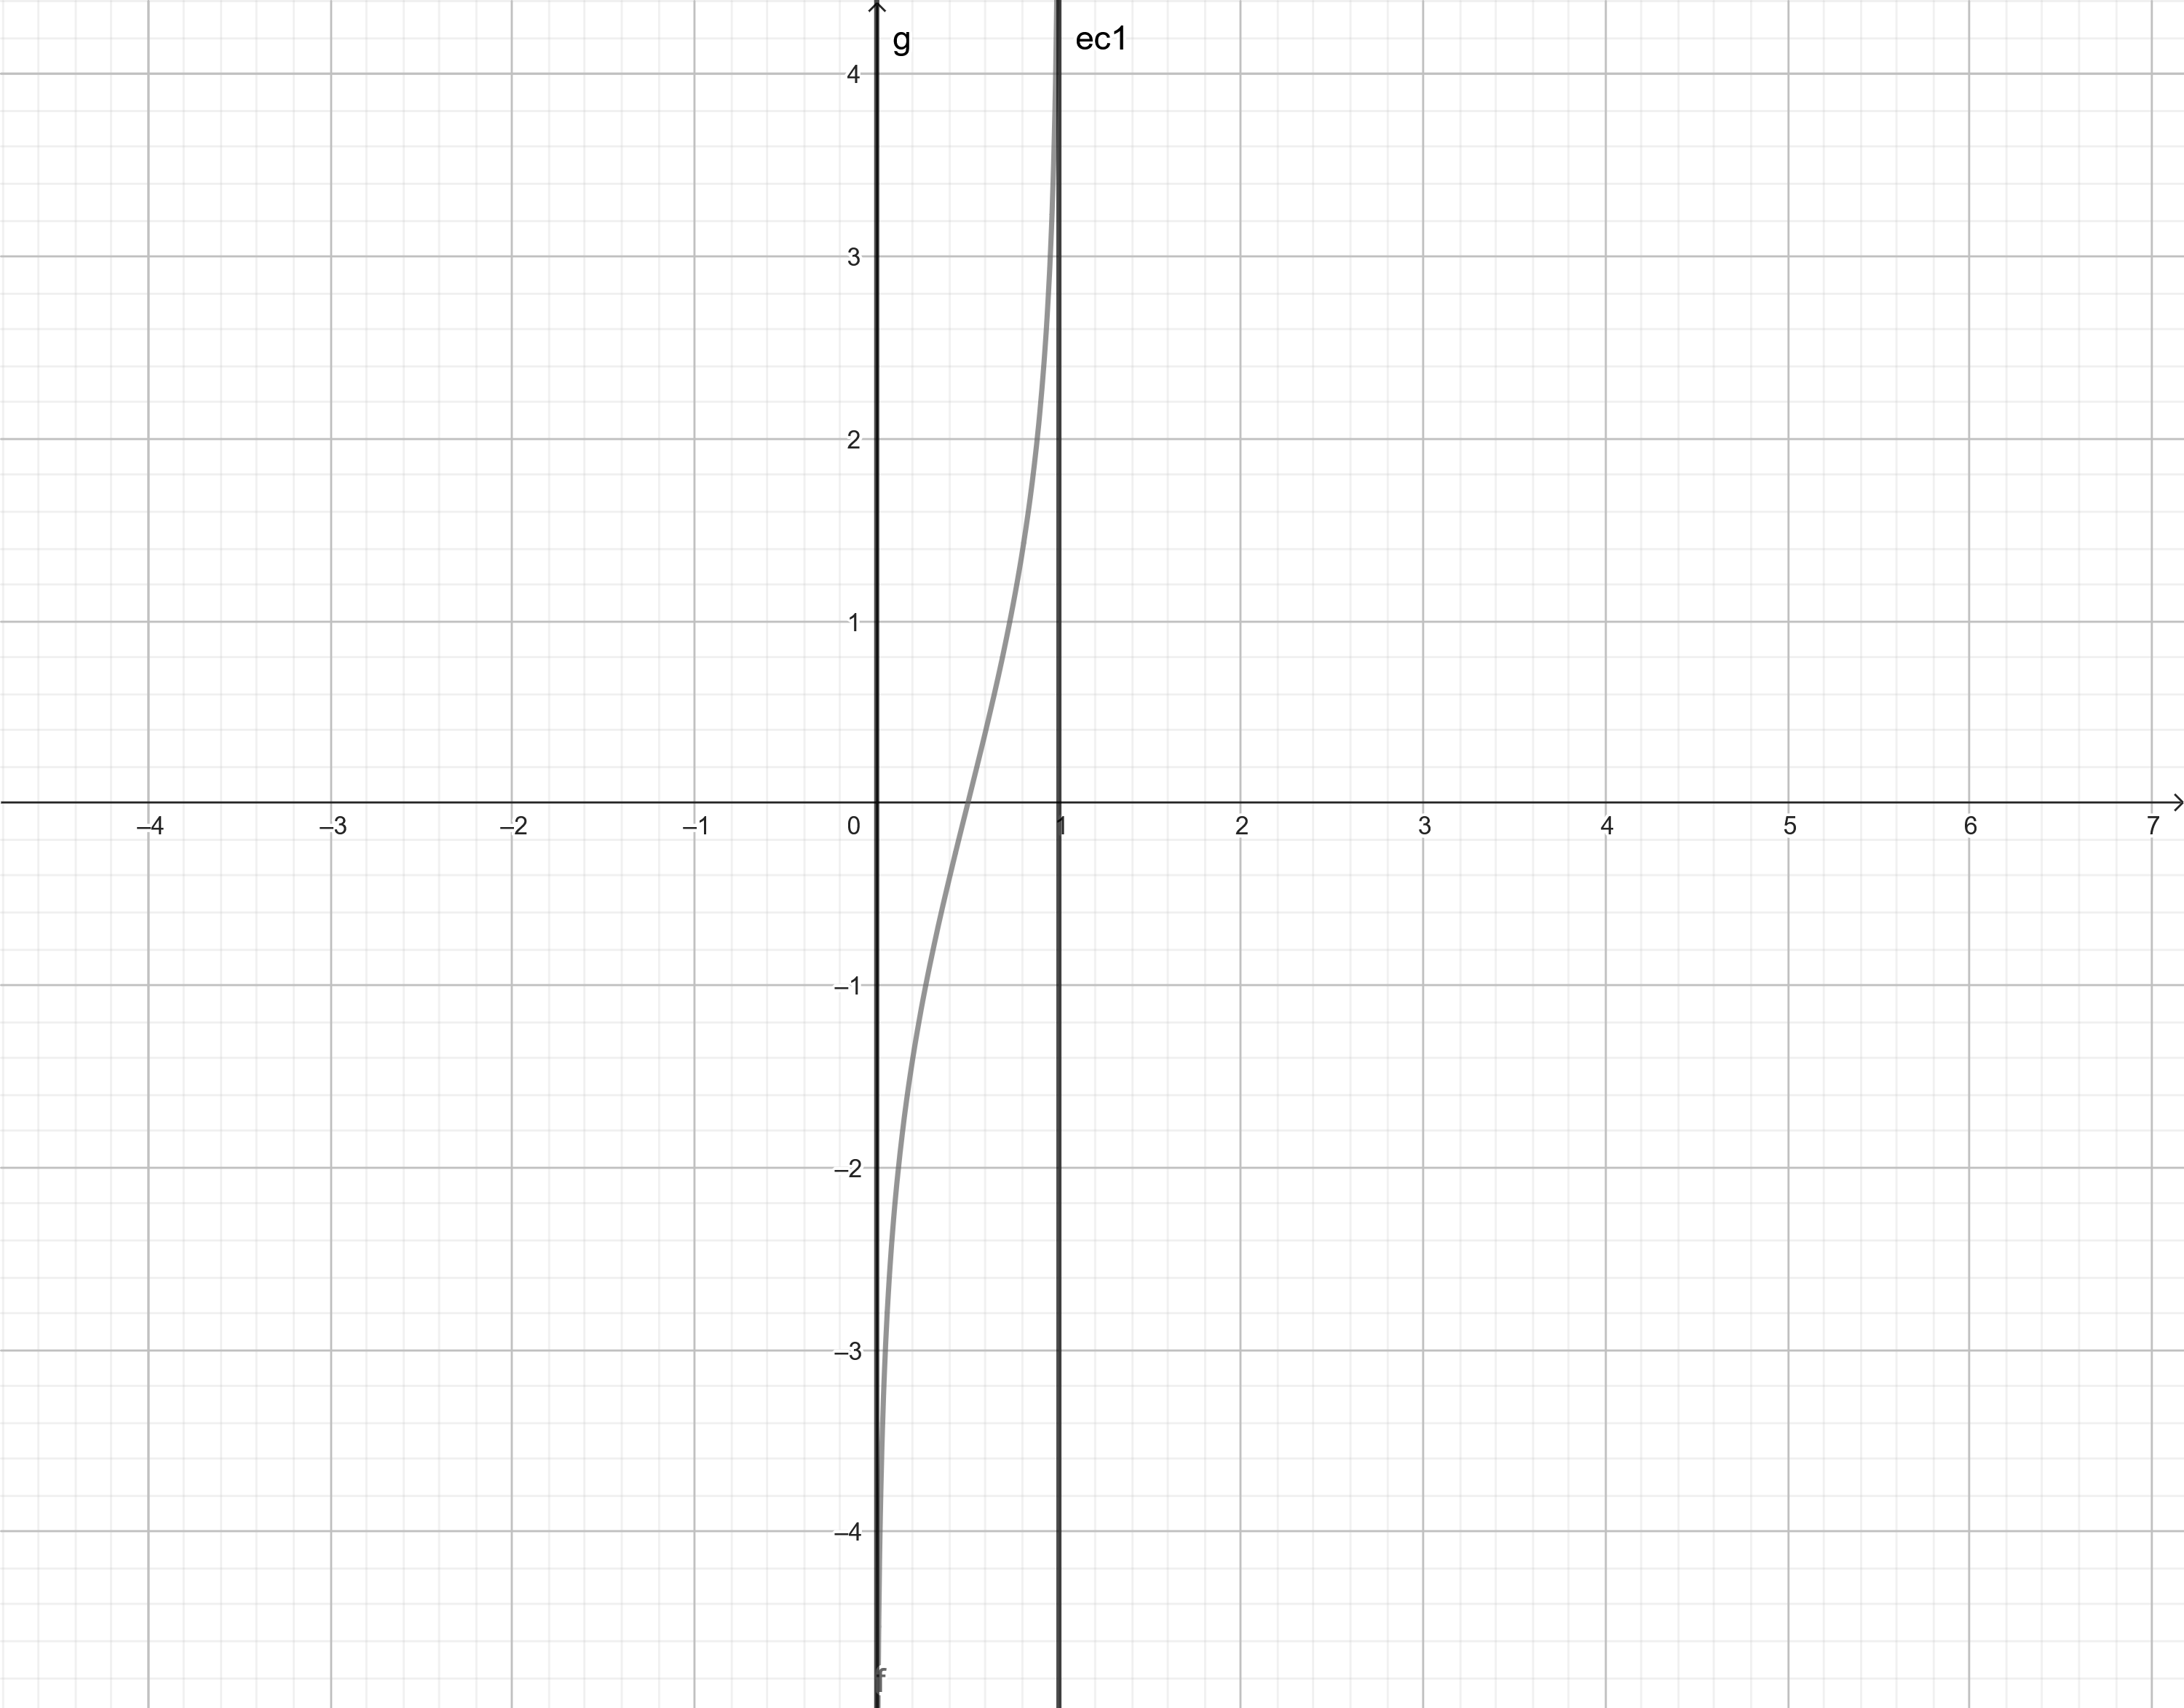
\includegraphics[width=0.5\linewidth]{Graficos/geogebra-export.png}
	\end{center}
	La imagen coincide con los números reales $\mathbb{R}$ por lo que contiene un conjunto abierto no trivial y por tanto el estadístico natural $\sum x_i$ es completo. 
}

Ahora veamos otro ejemplo en el que no se puede provocar la perteniencia a la familia exponencial: 

\ejemplo{
	Sea $X \sim U(\theta, 7\theta) \implies f_{\theta}(x) = \frac{1}{6\theta}\cdot I_{(\theta, 7\theta)}(x) \implies$
	$$f_{\theta}(\vec{x}) = \left(\frac{1}{6\theta}\right)^n \cdot I_{(\theta, 7\theta)}(x_{(1)}) \cdot I_{(\theta, 7\theta)}(x_{(n)})$$
	Entonces por el Teorema de Factorización de Fisher, tenemos que el estadístico $T(\vec{x}) = (x_{(1)}, x_{(n)})$ es suficiente.\\
	\begin{observación}
		Como la función indicadora depende de $\theta$, entonces la distribución no pertenece a la familia exponencial
	\end{observación}
	Recordemos además cuáles son las funciones de densidad de los máximos y lo mínimos (\underline{aunque en la práctica real hace falta demostrarlo siempre}): 
	$\begin{cases}
		f_{\theta}(x_{(n)}) = n(F_X(x))^{n-1} \cdot f_X(x) \\
		f_{\theta}(x_{(1)}) = n(1 - F_X(x))^{n-1} \cdot f_X(x)
	\end{cases} \implies$
	Saquemos primero la esperanza del máximo: \\
	$$E_{\theta}[x_{(n)}] = \int_{\theta}^{6\theta} x\cdot n\left(\frac{x - \theta}{6\theta}\right)^{n-1} \cdot \frac{1}{6\theta} = dx$$
	Para calcularla introduzcamos el cambio de variable: $\begin{cases} x = u \\ dv = f_{\theta}(x_{(n)}) \end{cases} \implies$
	$$ = \left[x \cdot \left(\frac{x - \theta}{6\theta}\right)^n\right]^{7\theta}_{x = \theta} - \int_{\theta}^{6\theta}\left(\frac{x - \theta}{6\theta}\right)^n dx$$

}


\begin{teorema}[Teorema de Basu]
	Si $T = T(X_1, \ldots, X_n)$ es un estadístico suficiente y completo y $U = U(X_1, \ldots, X_n)$ es un estadístico ancilario, entonces $T$ y $U$ son independientes
\end{teorema}

\begin{proof}
	Sea la muestra $(x_1, \ldots, x_n)$, un parámetro $\theta$ y sea un estadístico $T$ suficiente, entonces por definición tenemos que: 
	$$f(\vec{x} | T = t) \text{es indendiente de } \theta \implies$$
	$$f(U = u | T = t) = \sum_{\vec{x} : U(\vec{x}) = u} f(\vec{x} | T = t) \text{ es independiente de } \theta$$
	Aplicando las propiedades de los condicionales, tenemos que: 
	$$f_{\theta}(u) = f_{\theta}(t)f_{\theta}(u | t) \text{ pero como U es ancilario y T es completo, entonces:} \implies f(u) = f_{\theta}(t)f(u | t)$$

	Tomemos la función $h(t) = f(u | t) - f(u)$, entonces:
	$$E[h(T)] = E[f(u | T) - f(u)] = E[f(u | T)] - E[f(u)] = \int f(u | t)f(t)dt - \int f(u)f(t)dt = f(u) - f(u) = 0$$
	Entones como $T$ es completo, tenemos que $h(T) = 0$ c.s. $\implies f(u | t) = f(u) \implies$
	$$f(u | t) = \frac{f(u, t)}{f(t)} \iff f(t, u) = f(u)f(t) \implies U \text{ y } T \text{ son independientes}$$
\end{proof}

\ejemplo{
	Sea $X \sim U(0, \theta)$, veamos que $X_{(n)}$ y $\frac{X_{(1)}}{X_{(n)}}$ son independientes:\\
	$$ X \sim U(0, \theta) \implies f_{\theta}(x) = \frac{1}{\theta} \cdot I_{(0, \theta)}(x) \implies F_{X_{(n)}}(x) = P(X_{(n)} \leq x) = P(X_1 \leq x, \ldots, X_n \leq x) = $$ $$ = P(X_1 \leq x)\cdot \ldots \cdot P(X_n \leq x) = (F(x))^n = \left(\frac{x}{\theta}\right)^{n} \implies f_{\theta}(x) = n\left(\frac{x}{\theta}\right)^{n-1} \cdot \frac{1}{\theta} = \frac{n}{\theta^n}x^{n-1}$$
	Dado que por el Teorema de Factorización de Fisher, esta distribución es suficiente, consideraremos que $X_{(n)}$ es el estadístico suficiente y completo.\\
	Veamos ahora la función de densidad de $\frac{X_{(1)}}{X_{(n)}}$, para ello calculemos la función de densidad de $X_{(1)}$:
	$$F_{X_{(1)}}(x) = P(X_{(1)} \leq x) = 1 - P(X_{(1)} > x) = 1 - P(X_1 > x, \ldots, X_n > x) = $$ $$ = 1 - P(X_1 > x)\cdot \ldots \cdot P(X_n > x) = 1 - (1 - F(x))^n = 1 - \left(1 - \frac{x}{\theta}\right)^n \implies f_{\theta}(x) = n\left(1 - \frac{x}{\theta}\right)^{n-1} \cdot \frac{1}{\theta} = \frac{n}{\theta^n}(\theta - x)^{n-1}$$
}

\ejemplo{
	Sea una m.a.s. de tamaño $n$ de una población $X \sim N(\theta, \sigma)$ se tiene que: 
	$$\bar{X} \sim N(\mu, \frac{\sigma}{n}) \text{ ya que } \begin{cases} E[\bar{X}] = E\left[\frac{1}{n}\sum_{i = 1}^{n}X_i\right] = \frac{1}{n}\sum_{i = 1}^{n}E[X_i] = \frac{1}{n}n\theta = \theta \\ Var(\bar{X}) = Var\left(\frac{1}{n}\sum_{i = 1}^{n}X_i\right) = \frac{1}{n^2}\sum_{i = 1}^{n}Var(X_i) = \frac{1}{n^2}n\sigma = \frac{\sigma}{n} \end{cases}$$
	Y como se trata de una distribución perteneciente a la familia exponencial 2-paramétrica, entonces $\bar{X}$ es suficiente. Queda demostrar que sea completo, para ello, consideremos la función de densidad de $\bar{X}$:
	$$\bar{X} \sim N(\mu, \frac{\sigma}{n}) \implies f_{\theta}(x) = \sqrt{\frac{n}{2\pi\sigma}}e^{-\frac{n}{2\sigma}(x - \theta)^2}$$
	La completitud se da por definición. No obstante es una integral demasiado dificil de calcular, por lo que se puede deducir que $\bar{X}$ es completo. 
	Por el Teorema de Fisher sabemos que: 
	$$\frac{(n-1)S^2}{\sigma^2} \sim \chi^2(n-1) \implies S^2 \sim \frac{\sigma^2}{n-1}\chi^2(n-1) \implies S^2 \text{ es un estadístico ancilario} \implies$$
	Por el teorema de Basu, $\bar{X}$ y $S^2$ son independientes
}
    
    
\subsection{Principios de reducción de datos}

\begin{teorema}[Principio de verosimilitud]
	Dada una m.a.s. consideramos que la distribución de la muestra es una función de $\theta$ y no de la muestra en sí, es decir, $L(\theta | x_1, \ldots, x_n) = f(x_1, \ldots, x_n | \theta)$
\end{teorema}

\begin{proposición}
	Sean dos muestras $X = (x_1, \ldots, x_n)$ e $Y = (y_1, \ldots, y_m)$, si $\exists c(x, y)$ tal que $L_1(\theta | x) = c(x, y)L_2(\theta | y)$, entonces la evidencia estadística que suministran ambas muestras es idéntica. Es decir, $Ev(E_1, \vec{x}) = Ev(E_2, \vec{y})$
\end{proposición}

\ejemplo{
	Sea un modelo $Binomial(n, \theta)$ la evidencia que se obtiene del mismo, sobre $\theta$, cuando se observan $t$ éxitos en $n$ repeticiones, es la misma que la obtenida por un modelo $Binomial negativo(t, \theta)$, siempre que se suponga que se han realizado $n$ repeticiones hasta obtener $t$ éxitos.\\
	$$ \text{En el primer caso tenemos que: } 
	f(t|\theta) = \binom{n}{t}\theta^t(1 - \theta)^{n-t} $$ $$\text{ y en el segundo caso: } g(\text{n repeticiones hasta obtener t éxitos} | \theta) = \binom{n-1}{t-1}\theta^t(1 - \theta)^{n-t}$$
	Por tanto, se puede aplicar el principio de verosimilitud, tomando la constante $c(t, n) = \frac{n}{t}$. Es decir, si para estimar la probabilidad con la que sale cara una moneda, se tira ésta $n$ veces,  y es $t$ el numero de cara s que se han presentado (modelo binomial), se obtiene la misma evidencia para $\theta$, que si se repite el experimento hasta observar $t$ caras y para ello ha habido que realizar $n$ repeticiones (modelo binomial negativo)
}
 

\begin{proposición}[Principio de suficiencia]
	En un experimento $E = \left(\chi, \theta, \mathcal{P} = \{f(\vec{x}|\theta) : \theta \in \Theta\} \right)$, si $T = T(\vec{X})$ es un estadístico suficiente para $\theta$ y se tiene que $T(\vec{x}) = T(\vec{y})$, entonces las dos muetras $\vec{x}$ e $\vec{y}$ suministran la misma evidencia estadística, es decir, $Ev(E, \vec{x}) = Ev(E, \vec{y})$
\end{proposición}

\ejemplo{
	En un experimento consistente en la repetición de $n$ pruebas de Bernoulli, la evidencia estadística que se obtiene de dos puntos muestrales con el mismo número de éxitos es la misma.
}

\begin{proposición}[Principio de condicionalidad]
	El principio de condicionalidad dice que si un mecanismo aleatorio no depende del valor a determinar $\theta$, no proporciona evidencia sobre él. Es decir, si $T = T(\vec{X})$ es un estadístico suficiente para $\theta$ y $T(\vec{x}) = T(\vec{y})$, entonces las dos muestras $\vec{x}$ e $\vec{y}$ suministran la misma evidencia estadística, es decir, $Ev(E, \vec{x}) = Ev(E, \vec{y})$
\end{proposición}

\ejemplo{
	Dados dos experimentos $E_1 = (\chi^n, f_1(\vec{x}|\theta))_{\theta \in \Theta \subset \mathbb{R}^{\ell}}$ y $E_2 = (\chi^m, f_2(\vec{y}|\theta))_{\theta \in \Theta \subset \mathbb{R}^{\ell}}$ y el lanzamiento de una moneda al aire representado por la v.a. $J$ tal que $P(J = 1) = P(J = 2) = \frac{1}{2}$, si $E = (\chi^n \cup \chi^m \times \{1, 2\}, f(\vec{x}, j|\theta))_{\theta \in \Theta \subset \mathbb{R}^{\ell}}$ es el experimento mixto representado por la v.a. $(Z, J)$ tal que $Z = \begin{cases} X & \text{ si } J = 1 \\ Y & \text{ si } J = 2 \end{cases}$, entonces $Ev(E, (\vec{x}, 1)) = Ev(E_1, \vec{x})$ y $Ev(E, (\vec{y}, 1)) = Ev(E_2, \vec{y})$
}
  
\begin{teorema}[Teorema de Birnbaum]
	El principio de verosimilitud es equivalente a los principios de suficiencia y condicionalidad.
\end{teorema}  

\subsection{Ejercicios}
\begin{problem}{2.1}
	Sea $X$ muestra de una población $N(0, \sigma)$, ¿Es $|X|$ un estadístico suficiente?
\end{problem}
\begin{sol}
	
\end{sol}